\section{Modularer Architekturvorschlag}
\label{sec:architektur}

%Komponenten des Brokers.
%
%
%In der CMP: Polling oder Notification?
%
%Was löst eine Aktion aus?
%- Monitoring der Services
%- Änderung der Umgebung
%- User-Aktion
%- Ergebnis einer anderen Policy

%Regelkreis: Soll- (Template) und Istzustand (Cloud-Deployment).

\begin{figure}
	\centering	
	\def\svgwidth{0.95\textwidth}
	{\tiny \textsf{
	\includesvg{images/broker-cycle}}}
%	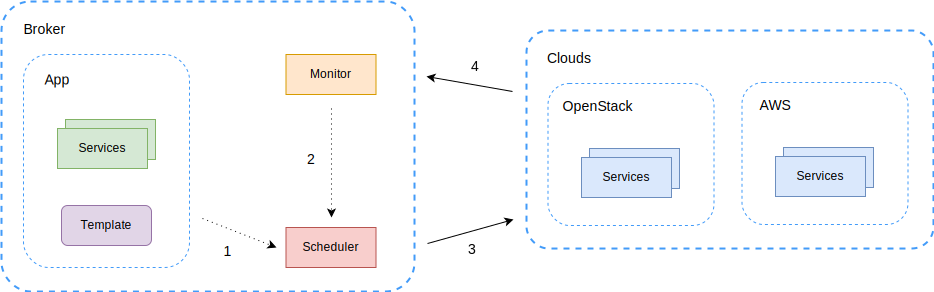
\includegraphics[width=\linewidth]{images/broker-cycle}
	\caption{Arbeitsweise des Multi-Cloud-Brokers als Regelkreis: (1) Sammeln der Meta-Informationen aller Cloud-Provider, (2) Sammeln der Laufzeitinformationen der Anwendungen, (3) Sammeln der SLAs, (4) Nutzeränderungen: Neue Anwendungen oder Anpassung von SLAs, (5) Optimierungsplanung, (6) Planausführung auf den Cloud-Infrastrukturen}
	\label{fig:cycle}
\end{figure}


\begin{minipage}[b]{0.45\linewidth}
\begin{flushleft}
\begin{enumerate}
\item Monitoring Cloud-Ressourcen
\begin{enumerate}
	\item Kapazität% (CPU, RAM, HDD, Netzwerk)
	\item Features% (Verschlüsselung, CUDA, \ldots)
	\item Geo-Lokation
	\item Preis
\end{enumerate}
\item Laufzeitinformationen% der PaaS/Anwendungen
\begin{enumerate}
	\item Auslastung
	\item Fehler
	\item Ausfälle
\end{enumerate}
\item Sammeln der SLAs
\begin{enumerate}
	\item Policy-Definitionen
	\item Policy-Konfiguration
	\item Placement-Algorithmen
\end{enumerate}
\end{enumerate}
\end{flushleft}
\end{minipage}
%
\hspace{0.5cm}
%
\begin{minipage}[b]{0.45\linewidth}	
\begin{enumerate}
\setcounter{enumi}{3}
\item (Neue Anwendung)
\item (Änderung von SLAs)
\item Optimierung
\begin{enumerate}
	\item Feste Vorgaben% (Geo, Backup)
	\item Weiche Kriterien% (Preis, Latenz, Verfügbarkeit)
\end{enumerate}
\item Ausführung
\begin{enumerate}
	\item Netzwerkkonfiguration
	\item Allokation/De-Allokation von Ressourcen
	\item Deployment
	\item Migration
	\item Logging% und \newline Benachrichtigung
	\item Backup
\end{enumerate}
\end{enumerate}
\end{minipage}

	
